%	proofeg.tex	(An example file for proof.sty)
%
%		Mar 6, 1997
%		Makoto Tatsuta
%
%	I hope you can learn how to use proof figure macros easily
%	by these examples.


\def\imp{\to}
\def\land{\mathbin\&}
% for LaTeX 2e naitive mode.
\documentclass[]{article}
\usepackage{proof}
\usepackage{tikz}
\usepackage{rotating}
\usepackage{enumitem}
\usepackage{mathtools, amssymb}
\usetikzlibrary{trees}
\usetikzlibrary{positioning}

\tikzset{%
  zeroarrow/.style = {-stealth,dashed},
  onearrow/.style = {-stealth,solid},
  c/.style = {circle,draw,solid,minimum width=2em,
        minimum height=2em},
  r/.style = {rectangle,draw,solid,minimum width=2em,
        minimum height=2em}
}
\begin{document}

\section{Predicates and interpretation}
\subsection{}
$$
\phi = \forall c.(\exists s.(\forall s'.(\neg att(s',c)\wedge eq(s,s')))\rightarrow can(c))
$$
$$I = <\{students, classes\},\{att, eq, can\}, \{\}>$$
Where $students$ is the set of all students $classes$ is the set of all classes.\\
$att(s,c)$ returns TRUE if student $s$ attends class $c$.\\
$eq(a,b)$ returns TRUE if student $a$ and $b$ are the same student.\\
$can(c)$ returns TRUE if course $c$ is cancelled.
\subsection{}
$$\phi = \forall p(\exists p'.\forall t.d(p,p',t) \wedge \exists t.\forall p'.d(p,p',t) \wedge \neg\forall p'.\forall t.d(p,p',t))$$
$$I = <\{people, times\}, \{d\}, \{\}>$$
where $people$ is the set of all people, $times$ is the set of all moments/time and $d(x,y,z)$ returns TRUE if person $x$ can deceive person $y$ at moment $z$.
\subsection{}
$$
\phi = \exists c.(h(c)\wedge \exists c'.(h(c') \wedge \neg eq(c,c')\wedge \forall c''.(\neg h(c'')\vee eq(c,c'')\vee eq(c',c''))))
$$
$$
I = <\{cats\},\{h, eq\}, \{\}>
$$
Where $cats$ is the set of all cats.\\
h(c) returns TRUE if cat $c$ is in the house.\\
eq(a,b) returns TRUE if cat $a$ and $b$ are the same cat.
\section{Semantic Tableaux}

\begin{center}
$\neg\exists x.\forall y.((p(x,y) \wedge \neg p(y,x))\rightarrow (p(x,y) \rightarrow q(y,x)))$
\\$|$\\
$\neg\forall y.((p(a,y) \wedge \neg p(y,a))\rightarrow (p(a,y) \rightarrow q(y,a)))$
\\$|$\\
$\neg ((p(a,b) \wedge \neg p(b,a))\rightarrow (p(a,b) \rightarrow q(b,a)))$
\\$|$\\
$(p(a,b) \wedge \neg p(b,a)), \neg(p(a,b) \rightarrow q(b,a))
$\\$|$\\
$(p(a,b) \wedge \neg p(b,a)), p(a,b), \neg q(b,a)$
\\$|$\\
$p(a,b), \neg p(b,a), p(a,b), \neg q(b,a)$
\end{center}
\noindent Since there are open endings in the tableau for the negation of the given formula, we can conclude that the formula is not valid.\\
\\
From the open leaf we can construct the following interpretation:\\
\\
\begin{center}
$D = \{a,b\}$\\
$R_p = \{(a,b)\}$\\
$R_q = \emptyset$
\end{center}
\section{Deductive systems}

\subsection{Gentzen}
$$
\infer[\rightarrow_R]{\vdash\neg\exists x.\forall y.(p(x)\rightarrow q(y))\rightarrow\forall x. \exists y.(p(x)\wedge \neg q(y))}{
\infer[\neg_L]{\neg \exists x.\forall y(p(x)\rightarrow q(y)\vdash \forall x.\exists y.(p(x)\wedge \neg q(y))}{
\infer[\forall_R]{\vdash \exists x.\forall y.(p(x)\rightarrow q(y), \forall x.\exists y.(p(x)\wedge \neg q(y))}{
\infer[\exists_R]{\vdash \exists x.\forall y.(p(x)\rightarrow q(y), \exists y.(p(a)\wedge \neg q(y))}{
\infer[\forall_R]{\vdash \forall y.(p(a)\rightarrow q(y), \exists y.(p(a)\wedge \neg q(y))}{
\infer[\exists_R]{\vdash p(a)\rightarrow q(b), \exists y.(p(a)\wedge \neg q(y))}{
\infer[\rightarrow_R]{\vdash p(a)\rightarrow q(b), p(a)\wedge \neg q(b)}{
	\infer[\wedge_R]{p(a)\vdash q(b),p(a)\wedge\neg q(b)}{
		\infer{p(a)\vdash q(b),p(a)}{Axiom}
		&
		\infer[\neg_R]{p(a)\vdash q(b),\neg q(b)}{
			\infer{p(a),q(b)\vdash q(b)}{Axiom}
		}
	}
}
}}}}}}
$$
\subsection{Hilbert}
\section{Resolution}


Case in First Order Logic: \\
$
\forall x.((f(x)\vee d(x))\wedge (f(x) \rightarrow \neg l(x,C))\wedge (d(x)\rightarrow l(x,R))) \hspace{10pt}\wedge \\
\forall y.((l(E,y) \leftrightarrow\neg l(B,y)) \wedge l(B,y)) \hspace{10pt}
$\\
$I = <\{members, genres\},\{f,d,l\},\{B,E,C,R\}>$ \\ \\
B, E, C, R are constants for respectively Bob, Ellen, Comedy movies and Romance movies. \\
f(x) returns TRUE if (and only if) x is a fighter.\\
d(x) returns TRUE if (and only if)x is a dancer.\\
l(x,y) returns TRUE if (and only if) member x likes movie genre y.\\ \\
Query in First Order Logic: $\exists x.(f(x) \wedge \neg d(x))$\\ \\
In order to proof that there exists a fighter that is not a dancer we negate the query and use resolution to show that the negated query is not satisfiable.\\ \\
$
\forall x.((f(x)\vee d(x))\wedge (f(x) \rightarrow \neg l(x,C))\wedge (d(x)\rightarrow l(x,R))) \hspace{10pt}\wedge \\
\forall y.((l(E,y) \leftrightarrow\neg l(B,y)) \wedge l(B,y)) \hspace{10pt} \wedge \\
\neg\exists x.(f(x) \wedge \neg d(x))\\ \\
$
Separate identifiers:  \\
$
\forall x.((f(x)\vee d(x))\wedge (f(x) \rightarrow \neg l(x,C))\wedge (d(x)\rightarrow l(x,R))) \hspace{10pt}\wedge \\
\forall y.((l(E,y) \leftrightarrow\neg l(B,y)) \wedge l(B,y)) \hspace{10pt} \wedge \\
\neg\exists z.(f(z) \wedge \neg d(z))\\ \\
$
Convert operators:\\
$
\forall x.((f(x)\vee d(x))\wedge (\neg f(x) \vee \neg l(x,C))\wedge (\neg d(x)\vee l(x,R))) \hspace{10pt}\wedge \\ 
\forall y.((\neg l(E,y) \vee \neg l(B,y)) \wedge (l(B,y) \vee l(E,y)) \wedge l(B,y))
\hspace{10pt} \wedge\\
\neg\exists z.(f(z) \wedge \neg d(z))\\ \\
$
Push negation inward:\\
$
\forall x.((f(x)\vee d(x))\wedge (\neg f(x) \vee \neg l(x,C))\wedge (\neg d(x)\vee l(x,R))) \hspace{10pt}\wedge \\
\forall y.((\neg l(E,y) \vee \neg l(B,y)) \wedge (l(B,y) \vee l(E,y)) \wedge l(B,y))\hspace{10pt} \wedge\\
\forall z.(\neg f(z) \vee d(z))\\ \\
$
Extract quantifiers:\\
$
\forall x.\forall y.\forall z.(f(x)\vee d(x))\wedge (\neg f(x) \vee \neg l(x,C))\wedge (\neg d(x)\vee l(x,R)) \hspace{10pt}\wedge \\
(\neg l(E,y) \vee \neg l(B,y)) \wedge (l(B,y) \vee l(E,y)) \wedge l(B,y)\hspace{10pt}\\ \wedge
(\neg f(z) \vee d(z))\\ \\
$
Clausal form:\\
$
fx\hspace{2pt}dx,\bar{f}x\hspace{2pt}\bar{l}xC,\bar{d}x\hspace{2pt}lxR,
\bar{l}Ey \hspace{2pt} \bar{l}By, lBy\hspace{2pt} lEy, lBy,
\bar{f}z \hspace{2pt} dz
$\\ \\
The resolution proving that the statement is unjustifiable is shown in \ref{fig:Res}.\\\\
Conclusion: Resolution shows that the query $\neg\exists x.(f(x) \wedge \neg d(x))$ is unjustifiable. This proofs that there exists a fighter that is not a dancer.


\begin{figure}[h]
\centering
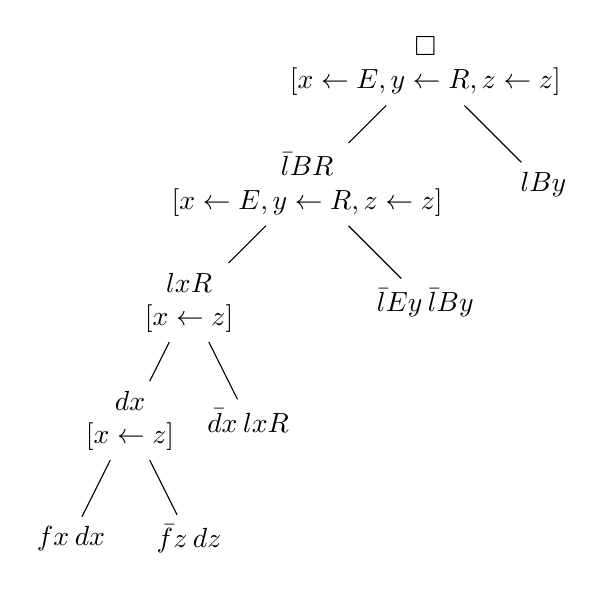
\begin{tikzpicture}[level distance=1.5cm,
  level 1/.style={sibling distance=3cm},
  level 3/.style={sibling distance=1.5cm},
  level 4/.style={sibling distance=1.5cm},
  node distance = 10cm]
  \node[align=center]{$\square$\\$[x\leftarrow E, y\leftarrow R, z\leftarrow z]$}
   child{node[align=center]{$\bar{l}BR$\\$[x\leftarrow E, y\leftarrow R, z\leftarrow z]$}
    child{ node[align=center]{$lxR$\\$[x\leftarrow z]$}
  	  child {node [align=center]{$dx$\\$[x\leftarrow z]$}
        child {node[align=center] {$fx\hspace{2pt}dx$}}
        child {node[align=center] {$\bar{f}z\hspace{2pt}dz$}}
      }
      child{node[align=center]{$\bar{d}x\hspace{2pt}lxR$}}
    }
    child{node[align=center]{$\bar{l}Ey\hspace{2pt}\bar{l}By$}}
   }
   child{node[align=center]{$lBy$}}
    ;
\end{tikzpicture}
\caption{Resolution for query $\neg\exists x.(f(x) \wedge\neg d(x)$} \label{fig:Res}
\end{figure}

\section{Job Interview}
\textbf{First candidate}:  his claim is incorrect. Kurt G\"odel has proven that it is impossible to capture all facts about natural number using the Peano axioms. His theory does not only work on the Peano axioms, but on all formal axiomatic systems for natural numbers.\\
\\
\textbf{Second candidate}:  his claim is partially correct. Using resolution it is possible to prove that a formula is unsatisfiable. This means that every interpretation falsifies that formula, so there is no doubt that the candidate can find an interpretation which falsifies that formula, but it would not be the resolution algorithm that gives him the interpretation. The resolution algorithm only proofs that it is not possible to satisfy all clauses of the clausal formula, but does not yield an interpretation which yields false.
\section{new}
\end{document}
